% Created by tikzDevice version 0.11 on 2018-04-09 15:27:55
% !TEX encoding = UTF-8 Unicode
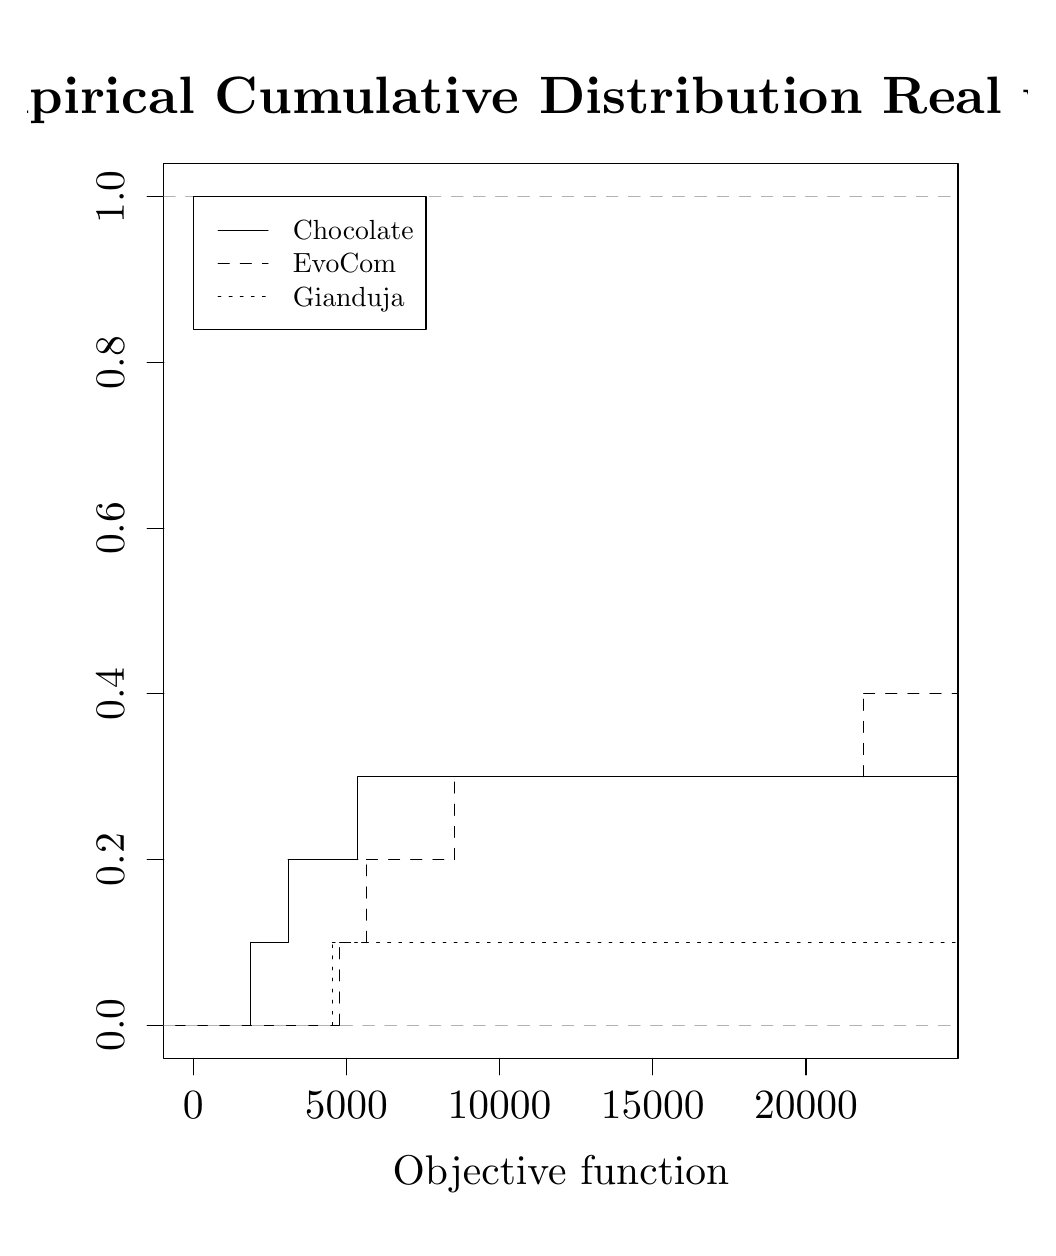
\begin{tikzpicture}[x=1pt,y=1pt]
\definecolor{fillColor}{RGB}{255,255,255}
\path[use as bounding box,fill=fillColor,fill opacity=0.00] (0,0) rectangle (361.35,433.62);
\begin{scope}
\path[clip] (  0.00,  0.00) rectangle (361.35,433.62);
\definecolor{drawColor}{RGB}{0,0,0}

\path[draw=drawColor,line width= 0.4pt,line join=round,line cap=round] ( 59.83, 61.20) -- (281.24, 61.20);

\path[draw=drawColor,line width= 0.4pt,line join=round,line cap=round] ( 59.83, 61.20) -- ( 59.83, 55.20);

\path[draw=drawColor,line width= 0.4pt,line join=round,line cap=round] (115.18, 61.20) -- (115.18, 55.20);

\path[draw=drawColor,line width= 0.4pt,line join=round,line cap=round] (170.53, 61.20) -- (170.53, 55.20);

\path[draw=drawColor,line width= 0.4pt,line join=round,line cap=round] (225.89, 61.20) -- (225.89, 55.20);

\path[draw=drawColor,line width= 0.4pt,line join=round,line cap=round] (281.24, 61.20) -- (281.24, 55.20);

\node[text=drawColor,anchor=base,inner sep=0pt, outer sep=0pt, scale=  1.50] at ( 59.83, 39.60) {0};

\node[text=drawColor,anchor=base,inner sep=0pt, outer sep=0pt, scale=  1.50] at (115.18, 39.60) {5000};

\node[text=drawColor,anchor=base,inner sep=0pt, outer sep=0pt, scale=  1.50] at (170.53, 39.60) {10000};

\node[text=drawColor,anchor=base,inner sep=0pt, outer sep=0pt, scale=  1.50] at (225.89, 39.60) {15000};

\node[text=drawColor,anchor=base,inner sep=0pt, outer sep=0pt, scale=  1.50] at (281.24, 39.60) {20000};

\path[draw=drawColor,line width= 0.4pt,line join=round,line cap=round] ( 49.20, 73.17) -- ( 49.20,372.45);

\path[draw=drawColor,line width= 0.4pt,line join=round,line cap=round] ( 49.20, 73.17) -- ( 43.20, 73.17);

\path[draw=drawColor,line width= 0.4pt,line join=round,line cap=round] ( 49.20,133.03) -- ( 43.20,133.03);

\path[draw=drawColor,line width= 0.4pt,line join=round,line cap=round] ( 49.20,192.88) -- ( 43.20,192.88);

\path[draw=drawColor,line width= 0.4pt,line join=round,line cap=round] ( 49.20,252.74) -- ( 43.20,252.74);

\path[draw=drawColor,line width= 0.4pt,line join=round,line cap=round] ( 49.20,312.59) -- ( 43.20,312.59);

\path[draw=drawColor,line width= 0.4pt,line join=round,line cap=round] ( 49.20,372.45) -- ( 43.20,372.45);

\node[text=drawColor,rotate= 90.00,anchor=base,inner sep=0pt, outer sep=0pt, scale=  1.50] at ( 34.80, 73.17) {0.0};

\node[text=drawColor,rotate= 90.00,anchor=base,inner sep=0pt, outer sep=0pt, scale=  1.50] at ( 34.80,133.03) {0.2};

\node[text=drawColor,rotate= 90.00,anchor=base,inner sep=0pt, outer sep=0pt, scale=  1.50] at ( 34.80,192.88) {0.4};

\node[text=drawColor,rotate= 90.00,anchor=base,inner sep=0pt, outer sep=0pt, scale=  1.50] at ( 34.80,252.74) {0.6};

\node[text=drawColor,rotate= 90.00,anchor=base,inner sep=0pt, outer sep=0pt, scale=  1.50] at ( 34.80,312.59) {0.8};

\node[text=drawColor,rotate= 90.00,anchor=base,inner sep=0pt, outer sep=0pt, scale=  1.50] at ( 34.80,372.45) {1.0};

\path[draw=drawColor,line width= 0.4pt,line join=round,line cap=round] ( 49.20, 61.20) --
	(336.15, 61.20) --
	(336.15,384.42) --
	( 49.20,384.42) --
	( 49.20, 61.20);
\end{scope}
\begin{scope}
\path[clip] (  0.00,  0.00) rectangle (361.35,433.62);
\definecolor{drawColor}{RGB}{0,0,0}

\node[text=drawColor,anchor=base,inner sep=0pt, outer sep=0pt, scale=  1.90] at (192.68,402.46) {\bfseries Empirical Cumulative Distribution Real values};

\node[text=drawColor,anchor=base,inner sep=0pt, outer sep=0pt, scale=  1.50] at (192.68, 15.60) {Objective function};
\end{scope}
\begin{scope}
\path[clip] ( 49.20, 61.20) rectangle (336.15,384.42);
\definecolor{drawColor}{RGB}{0,0,0}

\path[draw=drawColor,line width= 0.4pt,dash pattern=on 1pt off 3pt ,line join=round,line cap=round] (  0.00, 73.17) -- (110.12, 73.17);

\path[draw=drawColor,line width= 0.4pt,dash pattern=on 1pt off 3pt ,line join=round,line cap=round] (110.12,103.10) -- (361.35,103.10);

\path[draw=drawColor,line width= 0.4pt,dash pattern=on 1pt off 3pt ,line join=round,line cap=round] (110.12, 73.17) -- (110.12,103.10);
\definecolor{drawColor}{gray}{0.70}

\path[draw=drawColor,line width= 0.4pt,dash pattern=on 4pt off 4pt ,line join=round,line cap=round] ( 49.20, 73.17) -- (336.15, 73.17);

\path[draw=drawColor,line width= 0.4pt,dash pattern=on 4pt off 4pt ,line join=round,line cap=round] ( 49.20,372.45) -- (336.15,372.45);
\definecolor{drawColor}{RGB}{0,0,0}

\path[draw=drawColor,line width= 0.4pt,dash pattern=on 4pt off 4pt ,line join=round,line cap=round] ( 44.65, 73.17) -- (112.69, 73.17);

\path[draw=drawColor,line width= 0.4pt,dash pattern=on 4pt off 4pt ,line join=round,line cap=round] (112.69,103.10) -- (122.40,103.10);

\path[draw=drawColor,line width= 0.4pt,dash pattern=on 4pt off 4pt ,line join=round,line cap=round] (122.40,133.03) -- (154.27,133.03);

\path[draw=drawColor,line width= 0.4pt,dash pattern=on 4pt off 4pt ,line join=round,line cap=round] (154.27,162.95) -- (302.04,162.95);

\path[draw=drawColor,line width= 0.4pt,dash pattern=on 4pt off 4pt ,line join=round,line cap=round] (302.04,192.88) -- (361.35,192.88);

\path[draw=drawColor,line width= 0.4pt,dash pattern=on 4pt off 4pt ,line join=round,line cap=round] (112.69, 73.17) -- (112.69,103.10);

\path[draw=drawColor,line width= 0.4pt,dash pattern=on 4pt off 4pt ,line join=round,line cap=round] (122.40,103.10) -- (122.40,133.03);

\path[draw=drawColor,line width= 0.4pt,dash pattern=on 4pt off 4pt ,line join=round,line cap=round] (154.27,133.03) -- (154.27,162.95);

\path[draw=drawColor,line width= 0.4pt,dash pattern=on 4pt off 4pt ,line join=round,line cap=round] (302.04,162.95) -- (302.04,192.88);
\definecolor{drawColor}{gray}{0.70}

\path[draw=drawColor,line width= 0.4pt,dash pattern=on 4pt off 4pt ,line join=round,line cap=round] ( 49.20, 73.17) -- (336.15, 73.17);

\path[draw=drawColor,line width= 0.4pt,dash pattern=on 4pt off 4pt ,line join=round,line cap=round] ( 49.20,372.45) -- (336.15,372.45);
\definecolor{drawColor}{RGB}{0,0,0}

\path[draw=drawColor,line width= 0.4pt,line join=round,line cap=round] ( 11.29, 73.17) -- ( 80.59, 73.17);

\path[draw=drawColor,line width= 0.4pt,line join=round,line cap=round] ( 80.59,103.10) -- ( 94.14,103.10);

\path[draw=drawColor,line width= 0.4pt,line join=round,line cap=round] ( 94.14,133.03) -- (119.30,133.03);

\path[draw=drawColor,line width= 0.4pt,line join=round,line cap=round] (119.30,162.95) -- (361.35,162.95);

\path[draw=drawColor,line width= 0.4pt,line join=round,line cap=round] ( 80.59, 73.17) -- ( 80.59,103.10);

\path[draw=drawColor,line width= 0.4pt,line join=round,line cap=round] ( 94.14,103.10) -- ( 94.14,133.03);

\path[draw=drawColor,line width= 0.4pt,line join=round,line cap=round] (119.30,133.03) -- (119.30,162.95);
\definecolor{drawColor}{gray}{0.70}

\path[draw=drawColor,line width= 0.4pt,dash pattern=on 4pt off 4pt ,line join=round,line cap=round] ( 49.20, 73.17) -- (336.15, 73.17);

\path[draw=drawColor,line width= 0.4pt,dash pattern=on 4pt off 4pt ,line join=round,line cap=round] ( 49.20,372.45) -- (336.15,372.45);
\definecolor{drawColor}{RGB}{0,0,0}

\path[draw=drawColor,line width= 0.4pt,line join=round,line cap=round] ( 59.83,372.45) rectangle (143.93,324.45);

\path[draw=drawColor,line width= 0.4pt,line join=round,line cap=round] ( 68.83,360.45) -- ( 86.83,360.45);

\path[draw=drawColor,line width= 0.4pt,dash pattern=on 4pt off 4pt ,line join=round,line cap=round] ( 68.83,348.45) -- ( 86.83,348.45);

\path[draw=drawColor,line width= 0.4pt,dash pattern=on 1pt off 3pt ,line join=round,line cap=round] ( 68.83,336.45) -- ( 86.83,336.45);

\node[text=drawColor,anchor=base west,inner sep=0pt, outer sep=0pt, scale=  1.00] at ( 95.83,357.01) {Chocolate};

\node[text=drawColor,anchor=base west,inner sep=0pt, outer sep=0pt, scale=  1.00] at ( 95.83,345.01) {EvoCom};

\node[text=drawColor,anchor=base west,inner sep=0pt, outer sep=0pt, scale=  1.00] at ( 95.83,333.01) {Gianduja};
\end{scope}
\end{tikzpicture}
